\chapter{Conclusións}
\minitoc
\label{chap:conclusiones}
\vspace{0.5cm}

%%%%%%%%%%%%%%%%%%%%%%%%%%%%%%%%%%%%%%%%%%%%%%%%%%%%%%%%%%%%%%%%%%%%%%%%%%%%%%%%
% Objetivo: Contar cómo está ahora el proyecto, si ha merecido la              %
%           pena, lo que se ha aprendido, si se aplicaría de nuevo, etc.       %
%%%%%%%%%%%%%%%%%%%%%%%%%%%%%%%%%%%%%%%%%%%%%%%%%%%%%%%%%%%%%%%%%%%%%%%%%%%%%%%%

\lettrine{N}{este} capítulo exporanse as conclusións do proxecto: desde as
múltiples incidencias, as maneiras de resolvelas e as leccións que se
aprenderon delas, ata as oportunidades de mellora ou futuras liñas de traballo.

\section{Incidencias durante o desenvolvemento do proxecto}

 \subsection{Planificación}

  \subsubsection{Xestión do proxecto}

  Como se comentou no capítulo \ref{chap:planificacion}, nun primeiro momento
  escolleuse \textit{OpenProj} coma xestor de proxectos, procedendo a meter
  nel toda a planificación. Todo ía ben, ata que un día fallou sen explicación
  aparente. \\

  Por motivos de dispoñibilidade de tempo do proxectando (estudos, traballo,
  etc.) decidiuse empregar un calendario de media xornada para o proxecto. Pois
  resulta que \textit{OpenProj}, alomenos na súa última versión liberada
  (v1.4-2, do 02/10/2008), presenta problemas á hora de manexar calendarios que
  non son o calendario por defecto (xornada completa). \\

  Concretamente, o erro deuse un día calquera ó abrir o ficheiro do proxecto
  cando, sen explicación aparante e sen ter cambiado nada, pasou de empregar un
  calendario de media xornada a un de xornada completa composto por dous de
  media xornada. É dicir, o que fixo foi meter nun mesmo día dúas medias
  xornadas e, polo tanto, reducir o intervalo estimado de datas á metade. A
  partires dese momento, aínda sen ter salvado os cambios, o erro reproducíase
  sempre. \\

  Dito problema non é salvable polo usuario de ningunha maneira sen
  distorsionar os datos da planificación, polo que é preciso corrixilo no
  código da aplicación. Investigando pola rede, parece ser que o erro estaba xa
  corrixido na seguinte versión, pero dita versión non era libre e non tiña
  visos de chegar a selo en moito tempo (\textit{OpenProj} tamén cunha versión
  comercial). \\

  Por dito motivo, tocou tirar coa planificación feita e volver comezar. Do que
  quedaba na lista e guiándose polas recomendacións, seleccionouse
  \textit{Planner}. \\

  \textit{Planner} é un xestor bastante sinxelo e rápido. Perdíase algo de
  funcionalidade fronte a \textit{OpenProj}, pero dado o atraso acumulado e que
  as pequenas carencias que se lle vían eran mitigables, optouse por el
  igualmente. \\

  Houbo que refacer toda a planificación de cero, dado que os formatos non eran
  compatibles e a xestión da información é totalmente diferente. \\

  Todo perfecto, ata que tocou asignar recursos materiais ás tarefas.
  Seleccionada a primeira tarefa, que xa tiña asignado un recurso humano,
  asígnaselle un recurso material e de repente a duración da tarefa redúcese á
  metade. É dicir, os recursos materiais consomen esforzo. En resumo, que os
  recursos materiais traballan. Para entenderse, se nunha tarefa se emprega,
  por exemplo, un paquete de folios, ese paquete traballa. Inadmisible. \\

  Isto pode ter sentido para recursos máquina, onde pode ser necesario
  contabilizar as horas de traballo da maquinaria, pero non para recursos
  materiais en xeral e sen posibilidade de decisión ó respecto.\\

  Notificáronse este e outros erros ós desenvolvedores, que procederon a
  marcalos todos coma duplicados, cando moitos deles non o eran e o resto tiñan
  un título moito máis descriptivo que os que xa había (polo que non se
  atoparon nunha busca previa). Ademais, agrupáronos todos nun único erro
  ``caixón de xastre'' sen relación. Por este último motivo e logo de que máis
  profesionais lles insistiran e non obtiveramos resposta algunha, desbotouse
  tamén o \textit{Planner}.\\

  Na lista restaban por probar \textit{GanttProject} e \textit{LibrePlan}.
  Analizando un pouco máis en profundidade o \textit{GanttProject} chegouse á
  conclusión de que era demasiado sinxelo (por non dicir incompleto) polo que
  se desbotou sen máis.\\

  Chegados a este punto, só quedaba \textit{LibrePlan}: servidor web, base de
  datos, interface web, multitude de opcións a priori complexas, xestión de
  información totalmente distinta a todo o visto anteriormente, alta curva de
  aprendizaxe e un longo etcétera.\\

  Volta outra vez a facer a planificación de cero. Ardua tarefa dada a
  lentitude da interface web. Tamén se detectou algún erro leve (corrixido en
  versións posteriores) e outro que parecía grave e ó final non era máis que o
  descoñecemento moi especifico que \textit{LibrePlan} marca por defecto e que
  se atopa bastante agochado. \\

  Con \textit{LibrePlan} deuse tamén unha incidencia grave, froito dun erro do
  entorno de escritorio do sistema operativo empregado. Nunha das múltiples
  actualizacións da aplicación, non se reconfigurou a base de datos por quedar
  oculta a fiestra de xestión da configuración, o que ocasionou que a
  aplicación se actualizase pero a base de datos non, facendo romper a primeira
  e corrompendo a segunda. \\

  Gracias ó traballo da xente detrás de \textit{LibrePlan} puido recuperarse a
  base de datos e con ela a planificación no mesmo estado que antes de
  corromperse.

 \subsection{Deseño do sistema}

  \subsubsection{Prototipo 3}

   \paragraph{Prototipo hardware}\mbox{}\\

    \subparagraph{Receptor XBee}\mbox{}\\

    Como se comentou no capítulo \ref{chap:diseno}, empregar un
    \textit{XBee Explorer USB} \cite{XBeeExplorer} (figura
    \ref{figura:XBeeExplorer}) como base do receptor XBee plantexaba un
    problema.

    \begin{figure}[htbp]
     \centering
     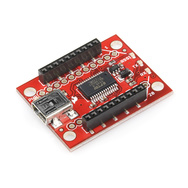
\includegraphics[scale=3.0,keepaspectratio=true]{./imagenes/xbee-explorer.jpg}
     % xbee-explorer.jpg: 188x188 pixel, 300dpi, 1.59x1.59 cm, bb=0 0 45 45
     \caption{XBee Explorer USB}
     \label{figura:XBeeExplorer2}
    \end{figure}

    Empregando esta placa, o dispositivo sería recoñecido no equipo coma un
    dispositivo USB, non coma un dispositivo MIDI, que é o que precisamos en
    última instancia. Por este motivo, habería que crear un controlador
    software para este dispostivo que fixese a conversión de USB a MIDI, para
    que puidese ser recoñecido polo sintentizador. Isto implicaría un retardo
    considerable (que seguramente dese ó traste co requisito de tempo real) e
    ademais, implicaría desenvolver un controlador distinto por cada familia de
    sistemas operativos. Como se pode intuir a simple vista, esta opción non
    era viable. \\

    Así que houbo que investigar un pouco para ver se había maneira de facer
    dita conversión por hardware, de tal maneira que ó enchufar o receptor vía
    USB fose recoñecido coma dispositivo MIDI, aforrando unha capa intermedia,
    un retardo importante e un esforzo máis ca considerable. \\

    Mirando o esquema do \textit{XBee Explorer USB} pódese ver que leva un chip
    \textit{FT232RL} (que é o que se encarga de facer a conversión de FTDI a
    USB) que, segundo pon aquí \cite{FT232RL} e aquí \cite{Moco}, non é posible
    reprogramar para facer unha conversión a MIDI. \\

    Segundo comentan tamén na segunda referencia, ese mesmo chip era o que se
    empregaba ata a versión \textit{Duemilanove} \cite{ArduinoDuemilanove} da
    placa estándar \textit{Arduino}, polo que tampouco era posible facelo con
    unha destas placas ata dita versión. \\

    A partires desa versión, cambiouse dito chip polos da familia
    \textit{Atmel Mega XuY} (8u2, 16u2, 32u4). Comezouse polo
    \textit{Arduino Uno} (8u2), que na súa terceira revisión o cambiou polo
    16u2 \cite{ArduinoUno}. E actualmente, a última placa que acaban de sacar,
    a \textit{Arduino Leonardo} \cite{ArduinoLeonardo} leva o 32u4. \\

    Dito chip está programado para funcionar exactamente igual que o
    \textit{FT232RL}, pero coa salvedade de que se pode reprogramar totalmente,
    polo que se pode empregar calquera placa \textit{Arduino} con dito chip
    para facer a conversión. \\

    Aínda que no momento de escribir estas liñas xa está dispoñible unha placa
    nova \cite{ArduinoLeonardo} que quizáis nos resultase máis sinxela de
    reprogramar, pois xa conta con USB nativo (sen necesidade de facer
    conversión serie-USB, polo que o novo firmware sería máis sinxelo), no
    momento de realizar o deseño hardware a última placa era a
    \textit{Arduino Uno r3}, que é un pouco máis completa, pero non conta con
    USB nativo. \\

    Sen embargo, se nos fixamos outra vez na referencia \cite{Moco}, vemos que
    xa a partires da revisión 2 (8u2) existe un firmware que fai este cometido,
    polo que se aforra moito tempo e esforzo. O esquema de funcionamento é o da
    figura \ref{figura:Moco2}.

    \begin{figure}[htbp]
     \centering
     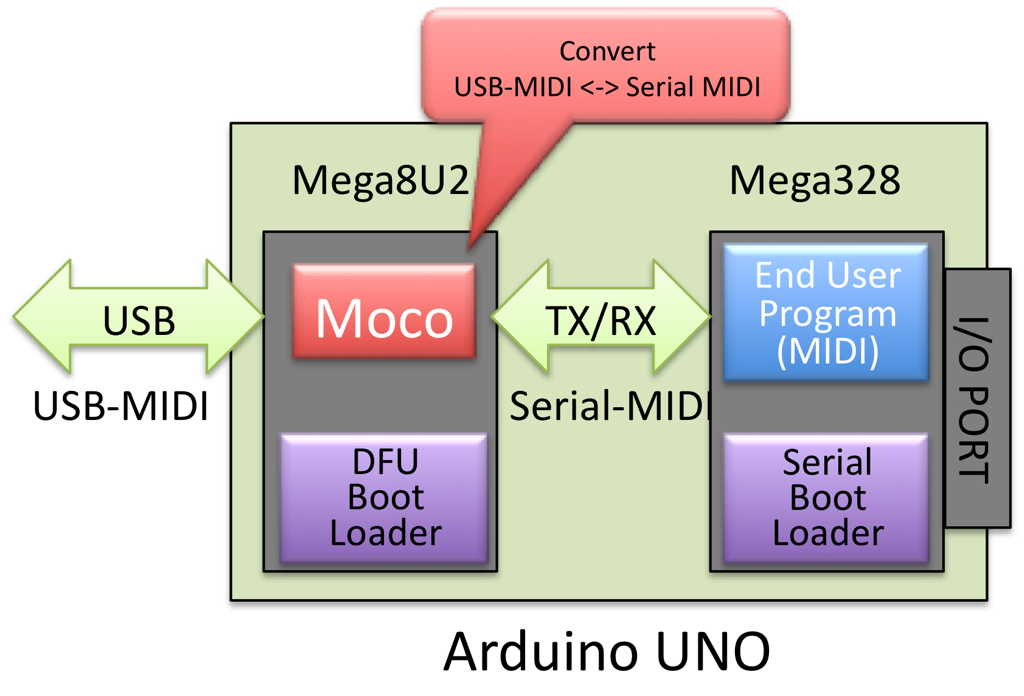
\includegraphics[scale=0.3,keepaspectratio=true]{./imagenes/moco.jpg}
     % moco.jpg: 1024x696 pixel, 72dpi, 36.12x24.55 cm, bb=0 0 1024 696
     \caption{Moco}
     \label{figura:Moco2}
    \end{figure}

    Ademais, polo que se pode ler ó final do artigo:

    \begin{quotation}
     \slshape
     Moco firmware can use as USB-MIDI \verb|<->| USB-Serial bridge with a 8u2
     or 32u4 board, like Adafruit’s 32u4 breakout board.
    \end{quotation}

    Vemos que dito firmware tamén funciona co chip 16u2 (que simplemente é un
    8u2 con máis memoria) e co 32u4 (que é o máis recente), polo que
    actualmente funciona con tódalas placas \textit{Arduino} lanzadas dende o
    \textit{Arduino Uno r2}. \\

    Polo que finalmente se optou por empregar como base do receptor un
    \textit{Arduino Uno} con firmware \textit{Moco}.

    \subparagraph{Fritzing}\mbox{}\\

    Como se comentou no capítulo \ref{chap:diseno}, a intalación de
    \textit{Fritzing} foi problemática. Instalada a versión dispoñible no
    repositorio da distribución en uso, comprobouse que a base de datos non
    contaba cunha gran cantidade de pezas. Procedeuse a comprobar a versión
    instalada (0.6.3) e cotexala coa última dispoñible nese momento (0.7.7b).
    Detectado o problema, intentouse compilar a versión dispoñible na web, pero
    non foi posible por mor de dependencias non localizables. A solución ó
    problema da escaseza de pezas da base de datos da versión do repositorio
    pasou por hackear a mesma, substituíndoa pola da versión máis recente (que
    contaba cun número de pezas moito máis elevado). \\

    Tamén se deron incidencias coas pezas a usar. A única reseñable por ter
    dado algo máis de traballo foi a que se deu co módulo de almacenamento, o
    \textit{MicroDrive G1}. \\

    Como se comentou no capítulo \ref{chap:diseno}, non estaba na base de datos
    do software por ser dun fabricante menos coñecido. Afortunadamente, estaba
    dispoñible no apartado de contribucións do repositorio da aplicación
    \cite{FioContribucionsFritzing}. Unha vez descargada, intentouse
    incorporala ó proxecto, pero non foi posible, pois tiña algún tipo de erro
    (e por iso non estaba incluida na base de datos). Investigando a fondo o
    ficheiro do proxecto (empregando un titorial \cite{TitorialFritzing} como
    guía), de formato \textit{fzp} (que non deixa de ser un XML) atopouse un
    erro na ruta ás diferentes vistas da peza (en formato svg), pois non
    coincidían totalmente os nomes dos ficheiros. Solventado o problema
    (hackeando o XML a man), procedeuse á súa incorporación ó proxecto. Así
    mesmo, notificouse o erro ós desenvolvedores da aplicación, contribuíndo a
    versión corrixida ó repositorio do proxecto \cite{ContribucionFritzing}.

\section{Conclusións finais}

 Lorem ipsum...